\documentclass{standalone}
\usepackage{tikz}
\usetikzlibrary{patterns, positioning}
\usepackage[sfdefault]{ClearSans} %% option 'sfdefault' activates Clear Sans as the default text font
\usepackage[T1]{fontenc}

\begin{document}
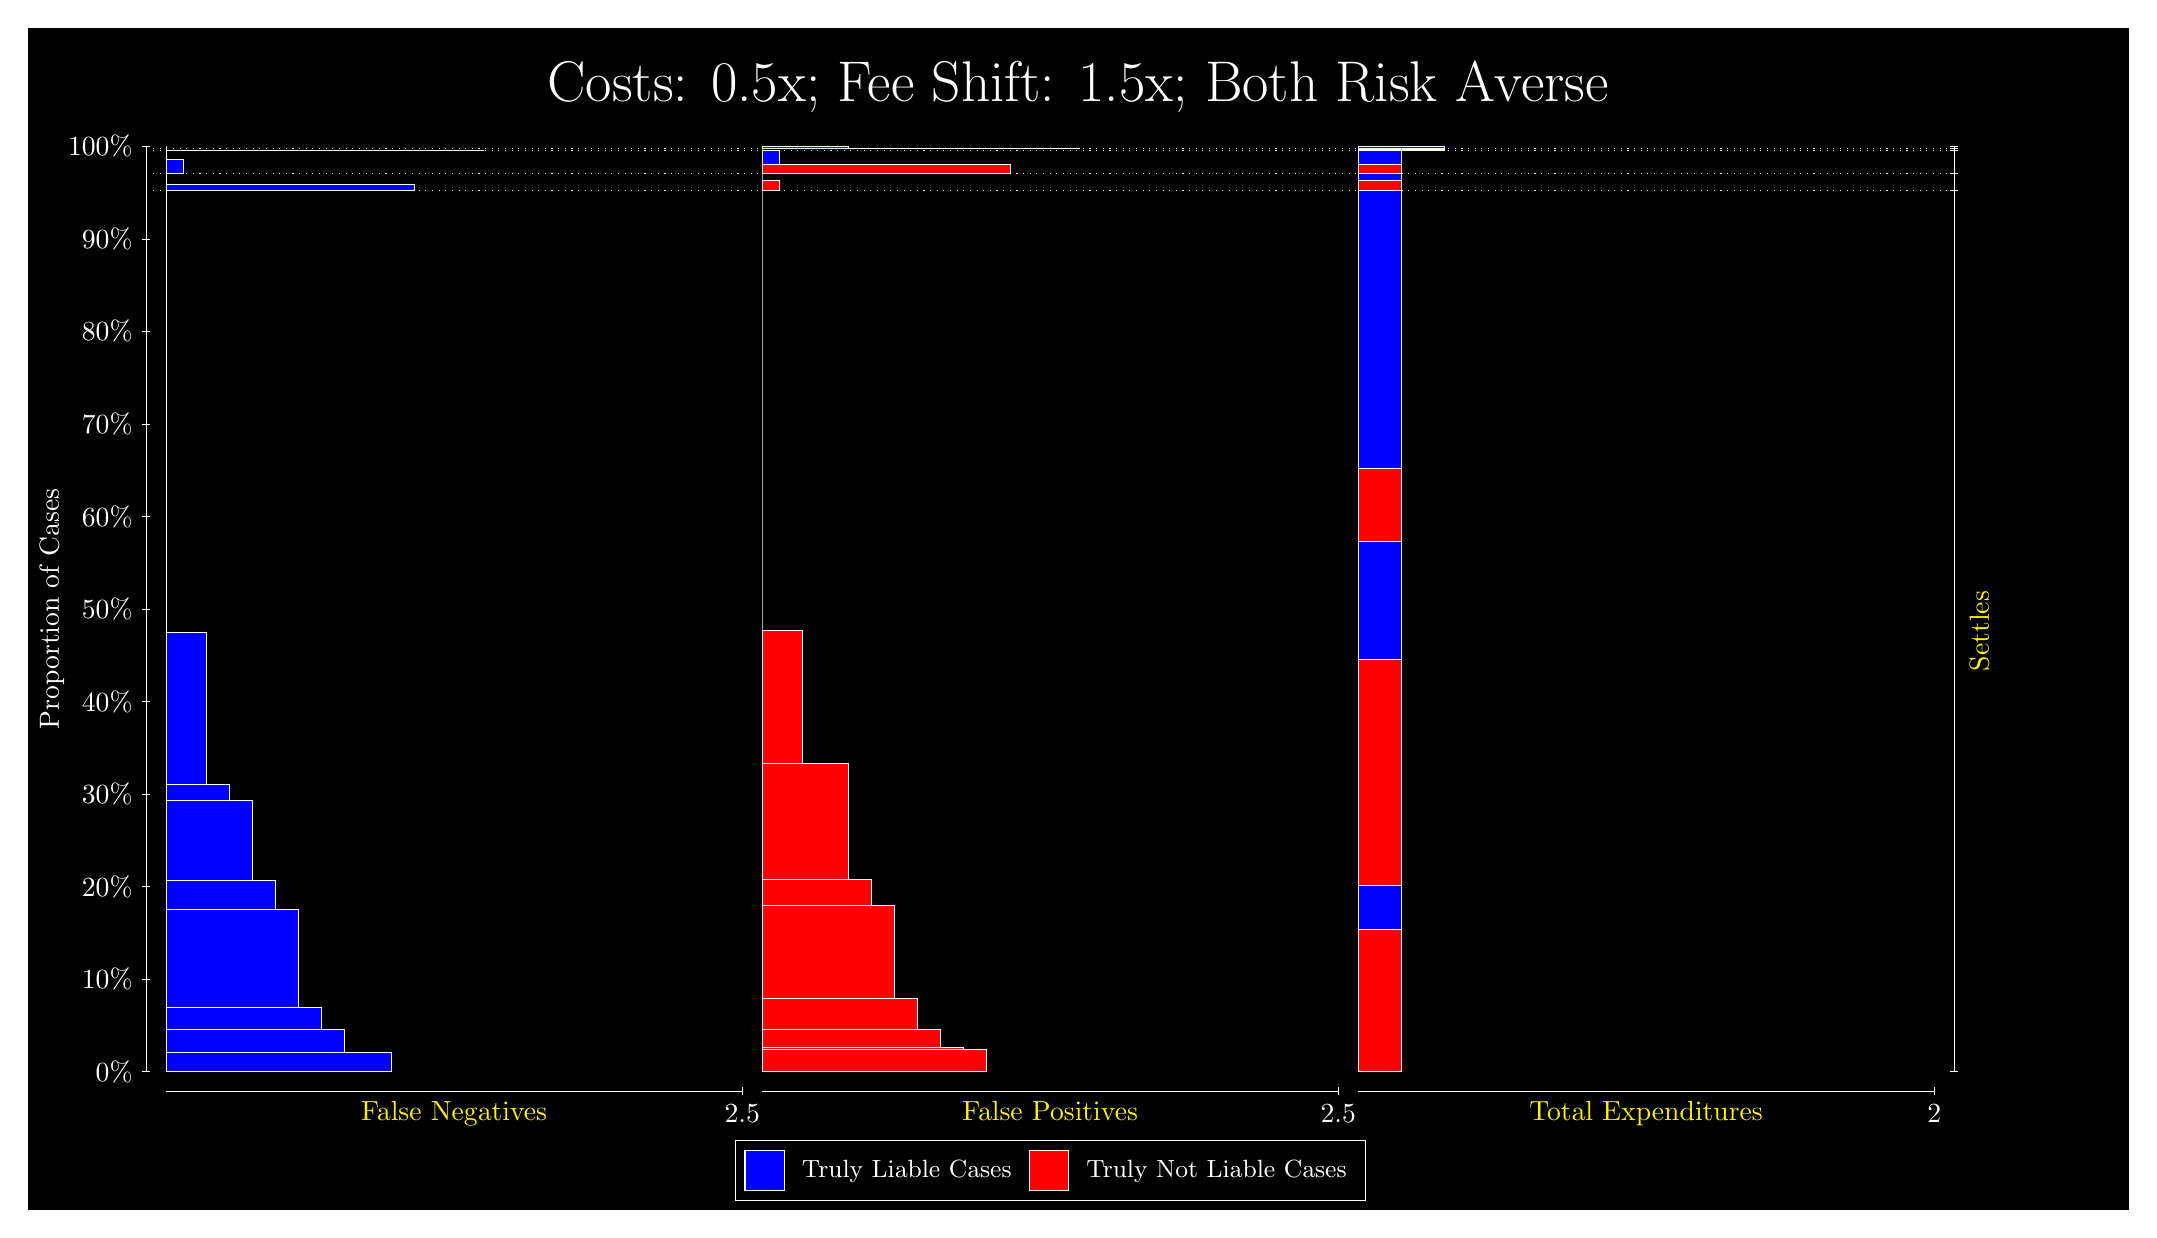
\begin{tikzpicture}
\draw[fill=black] (0,0) rectangle (26.667,15);
\draw[text=white] (0,13.5) rectangle (26.667,15) node[midway] {\huge Costs: 0.5x; Fee Shift: 1.5x; Both Risk Averse};
\draw[white, very thin] (1.5,1.75) -- (1.5,13.5);
\node[rotate=90, text=white, anchor=center] at (0.3, 7.625) {Proportion of Cases};
\draw[white, very thin] (1.45,1.75) -- (1.55,1.75);
\node[text=white, anchor=east] at (1.45, 1.75) {0\%};
\draw[white, very thin] (1.45,2.925) -- (1.55,2.925);
\node[text=white, anchor=east] at (1.45, 2.925) {10\%};
\draw[white, very thin] (1.45,4.1) -- (1.55,4.1);
\node[text=white, anchor=east] at (1.45, 4.1) {20\%};
\draw[white, very thin] (1.45,5.275) -- (1.55,5.275);
\node[text=white, anchor=east] at (1.45, 5.275) {30\%};
\draw[white, very thin] (1.45,6.45) -- (1.55,6.45);
\node[text=white, anchor=east] at (1.45, 6.45) {40\%};
\draw[white, very thin] (1.45,7.625) -- (1.55,7.625);
\node[text=white, anchor=east] at (1.45, 7.625) {50\%};
\draw[white, very thin] (1.45,8.8) -- (1.55,8.8);
\node[text=white, anchor=east] at (1.45, 8.8) {60\%};
\draw[white, very thin] (1.45,9.975) -- (1.55,9.975);
\node[text=white, anchor=east] at (1.45, 9.975) {70\%};
\draw[white, very thin] (1.45,11.15) -- (1.55,11.15);
\node[text=white, anchor=east] at (1.45, 11.15) {80\%};
\draw[white, very thin] (1.45,12.325) -- (1.55,12.325);
\node[text=white, anchor=east] at (1.45, 12.325) {90\%};
\draw[white, very thin] (1.45,13.5) -- (1.55,13.5);
\node[text=white, anchor=east] at (1.45, 13.5) {100\%};

\draw[white, very thin] (24.457,1.75) -- (24.457,13.5);
\draw[white, very thin] (24.407,1.75) -- (24.507,1.75);
\node[anchor=west] at (24.407, 1.75) {};
\draw[white, very thin] (24.407,12.938) -- (24.507,12.938);
\node[anchor=west] at (24.407, 12.938) {};
\draw[white, very thin] (24.407,13.158) -- (24.507,13.158);
\node[anchor=west] at (24.407, 13.158) {};
\draw[white, very thin] (24.407,13.445) -- (24.507,13.445);
\node[anchor=west] at (24.407, 13.445) {};
\draw[white, very thin] (24.407,13.472) -- (24.507,13.472);
\node[anchor=west] at (24.407, 13.472) {};
\draw[white, very thin] (24.407,13.5) -- (24.507,13.5);
\node[anchor=west] at (24.407, 13.5) {};

\draw[white, very thin, fill=blue] (1.75,1.75) rectangle (4.6044,1.9996);
\draw[white, very thin, fill=blue] (1.75,1.9996) rectangle (4.0188,2.2893);
\draw[white, very thin, fill=blue] (1.75,2.2893) rectangle (3.7261,2.5615);
\draw[white, very thin, fill=blue] (1.75,2.5615) rectangle (3.4333,3.8064);
\draw[white, very thin, fill=blue] (1.75,3.8064) rectangle (3.1406,4.1829);
\draw[white, very thin, fill=blue] (1.75,4.1829) rectangle (2.8478,5.201);
\draw[white, very thin, fill=blue] (1.75,5.201) rectangle (2.5551,5.3997);
\draw[white, very thin, fill=blue] (1.75,5.3997) rectangle (2.2623,7.3315);
\draw[white, very thin, fill=red] (1.75,7.3315) rectangle (1.75,12.938);
\draw[white, very thin, fill=blue] (1.75,12.938) rectangle (4.8971,13.024);
\draw[white, very thin, fill=red] (1.75,13.024) rectangle (1.75,13.158);
\draw[white, very thin, fill=blue] (1.75,13.158) rectangle (1.9696,13.338);
\draw[white, very thin, fill=red] (1.75,13.338) rectangle (1.75,13.445);
\draw[white, very thin, fill=blue] (1.75,13.445) rectangle (5.7754,13.454);
\draw[white, very thin, fill=red] (1.75,13.454) rectangle (1.75,13.472);
\draw[white, very thin, fill=red] (1.75,13.472) rectangle (1.75,13.481);
\draw[white, very thin, fill=blue] (1.75,13.481) rectangle (1.75,13.5);
\draw[white, very thin, fill=red] (9.3189,1.75) rectangle (12.173,2.0271);
\draw[white, very thin, fill=red] (9.3189,2.0271) rectangle (11.88,2.0585);
\draw[white, very thin, fill=red] (9.3189,2.0585) rectangle (11.588,2.292);
\draw[white, very thin, fill=red] (9.3189,2.292) rectangle (11.295,2.6805);
\draw[white, very thin, fill=red] (9.3189,2.6805) rectangle (11.002,3.8653);
\draw[white, very thin, fill=red] (9.3189,3.8653) rectangle (10.709,4.1915);
\draw[white, very thin, fill=red] (9.3189,4.1915) rectangle (10.417,5.6692);
\draw[white, very thin, fill=red] (9.3189,5.6692) rectangle (9.8312,7.3565);
\draw[white, very thin, fill=blue] (9.3189,7.3565) rectangle (9.3189,12.938);
\draw[white, very thin, fill=red] (9.3189,12.938) rectangle (9.5384,13.072);
\draw[white, very thin, fill=blue] (9.3189,13.072) rectangle (9.3189,13.158);
\draw[white, very thin, fill=red] (9.3189,13.158) rectangle (12.466,13.266);
\draw[white, very thin, fill=blue] (9.3189,13.266) rectangle (9.5384,13.445);
\draw[white, very thin, fill=red] (9.3189,13.445) rectangle (9.3189,13.463);
\draw[white, very thin, fill=blue] (9.3189,13.463) rectangle (9.3189,13.472);
\draw[white, very thin, fill=red] (9.3189,13.472) rectangle (13.344,13.481);
\draw[white, very thin, fill=blue] (9.3189,13.481) rectangle (10.417,13.5);
\draw[white, very thin, fill=red] (16.888,1.75) rectangle (17.437,3.5539);
\draw[white, very thin, fill=blue] (16.888,3.5539) rectangle (17.437,4.1158);
\draw[white, very thin, fill=red] (16.888,4.1158) rectangle (17.437,6.9879);
\draw[white, very thin, fill=blue] (16.888,6.9879) rectangle (17.437,8.4825);
\draw[white, very thin, fill=red] (16.888,8.4825) rectangle (17.437,9.4129);
\draw[white, very thin, fill=blue] (16.888,9.4129) rectangle (17.437,12.938);
\draw[white, very thin, fill=red] (16.888,12.938) rectangle (17.437,13.072);
\draw[white, very thin, fill=blue] (16.888,13.072) rectangle (17.437,13.158);
\draw[white, very thin, fill=red] (16.888,13.158) rectangle (17.437,13.266);
\draw[white, very thin, fill=blue] (16.888,13.266) rectangle (17.437,13.445);
\draw[white, very thin, fill=red] (16.888,13.445) rectangle (17.986,13.463);
\draw[white, very thin, fill=blue] (16.888,13.463) rectangle (17.986,13.472);
\draw[white, very thin, fill=red] (16.888,13.472) rectangle (17.986,13.481);
\draw[white, very thin, fill=blue] (16.888,13.481) rectangle (17.986,13.5);
\draw[white, dotted] (1.5,12.938) -- (24.457,12.938);
\draw[white, dotted] (1.5,13.158) -- (24.457,13.158);
\draw[white, dotted] (1.5,13.445) -- (24.457,13.445);
\draw[white, dotted] (1.5,13.472) -- (24.457,13.472);
\draw[white, very thin] (1.75,1.5) -- (9.0689,1.5);
\node[text=yellow, anchor=north] at (5.4094, 1.5) {False Negatives};
\draw[white, very thin] (9.0689,1.45) -- (9.0689,1.55);
\node[text=white, anchor=north] at (9.0689, 1.45) {2.5};

\draw[white, very thin] (9.3189,1.5) -- (16.638,1.5);
\node[text=yellow, anchor=north] at (12.978, 1.5) {False Positives};
\draw[white, very thin] (16.638,1.45) -- (16.638,1.55);
\node[text=white, anchor=north] at (16.638, 1.45) {2.5};

\draw[white, very thin] (16.888,1.5) -- (24.207,1.5);
\node[text=yellow, anchor=north] at (20.547, 1.5) {Total Expenditures};
\draw[white, very thin] (24.207,1.45) -- (24.207,1.55);
\node[text=white, anchor=north] at (24.207, 1.45) {2};

\node[text=yellow, centered, rotate=90] at (24.777, 7.344) {Settles};





\draw (12.978300999999998,1.5) node[draw=none] (baseCoordinate) {};
\begin{scope}[align=center]
        \matrix[scale=0.5, draw=white, below=0.5cm of baseCoordinate, nodes={draw}, column sep=0.1cm]{
            \node[rectangle, draw, minimum width=0.5cm, minimum height=0.5cm, fill=blue] {}; &
            \node[draw=none, font=\small, text=white] (B) {Truly Liable Cases}; &
            \node[rectangle, draw, minimum width=0.5cm, minimum height=0.5cm, fill=red] {}; &
            \node[draw=none, font=\small, text=white] (B) {Truly Not Liable Cases}; \\
            };
\end{scope}

\end{tikzpicture}
\end{document}